%%%%%%%%%%%%%%%%%%%%%%%%%%%%%%%%%
% ammana.es | Manual de cliente %
%                               %
%  Made with ❤️  by NoLegalTech  %
%%%%%%%%%%%%%%%%%%%%%%%%%%%%%%%%%

\documentclass[12pt, spanish]{article}

\usepackage{geometry}
\geometry{a4paper}

\usepackage{graphicx}
\graphicspath{{img/}}

\usepackage{adjustbox}

\usepackage{float}
\usepackage{wrapfig}

\usepackage[spanish]{babel}
\selectlanguage{spanish}

\usepackage[utf8]{inputenc}

\usepackage{enumitem}

\linespread{1.2}

\setlength{\parindent}{2em}
\setlength{\parskip}{1em}

\usepackage{concmath}
\usepackage[T1]{fontenc}

\usepackage{fancyhdr}

\fancyhf{}
\fancyhead[L]{
\includegraphics[height=5.0mm]{logo}}

\newlist{steps}{enumerate}{1}
\setlist[steps]{label={\arabic*)}}

\setlength{\headheight}{7.50mm}
\pagestyle{fancy}

%----------------------------------------------------------------------------------------

\begin{document}

%----------------------------------------------------------------------------------------

    \begin{titlepage}
        \newcommand { \HRule } { \rule {\linewidth} {0.5mm} }
        \center
        \textsc {\LARGE ammana.es} \\ [1.5cm]
        \HRule \\ [0.4cm]
        { \huge \bfseries Manual del administrador } \\ [0.4cm]
        \HRule \\ [1.5cm]
        { \large \today } \\ [3cm]
        \vfill
    \end{titlepage}

%----------------------------------------------------------------------------------------

    \tableofcontents

    \newpage

%----------------------------------------------------------------------------------------
    \section{Introducción}

        \textbf{ammana.es} funciona de forma prácticamente autónoma y los clientes pueden
        comprar y descargar protocolos sin intervención del administrador. La única
        excepción es cuando algún cliente paga por transferencia bancaria, en cuyo
        caso el pago debe ser marcado como cobrado de forma manual para que el cliente
        pueda descargarse el protocolo.

        Por otro lado, el panel de administración de \textbf{ammana.es}, junto con los de \textbf{Paypal} y
        \textbf{Quaderno}, dan acceso al administrador a la lista de clientes, facturas, pedidos, etc
        para su consulta, bien por curiosidad bien para ofrecer soporte a un cliente..

        Es decir, las funciones del administrador son 2:

        \begin{steps}
          \item Marcar como cobrados los pedidos que han sido pagados por transferencia
          \item Acceder a la información de clientes y facturas
        \end{steps}

%----------------------------------------------------------------------------------------
    \section{Acceso al panel de administración}

    Para acceder al panel de administración, simplemente debes hacer login con las credenciales
    del usuario, administrador. Es decir:

    \begin{steps}
        \item Click en ``Identificarse'':

            \medskip
            \begin{minipage}[t]{\linewidth}
            \raggedright
            \adjustbox{valign=t}{%
                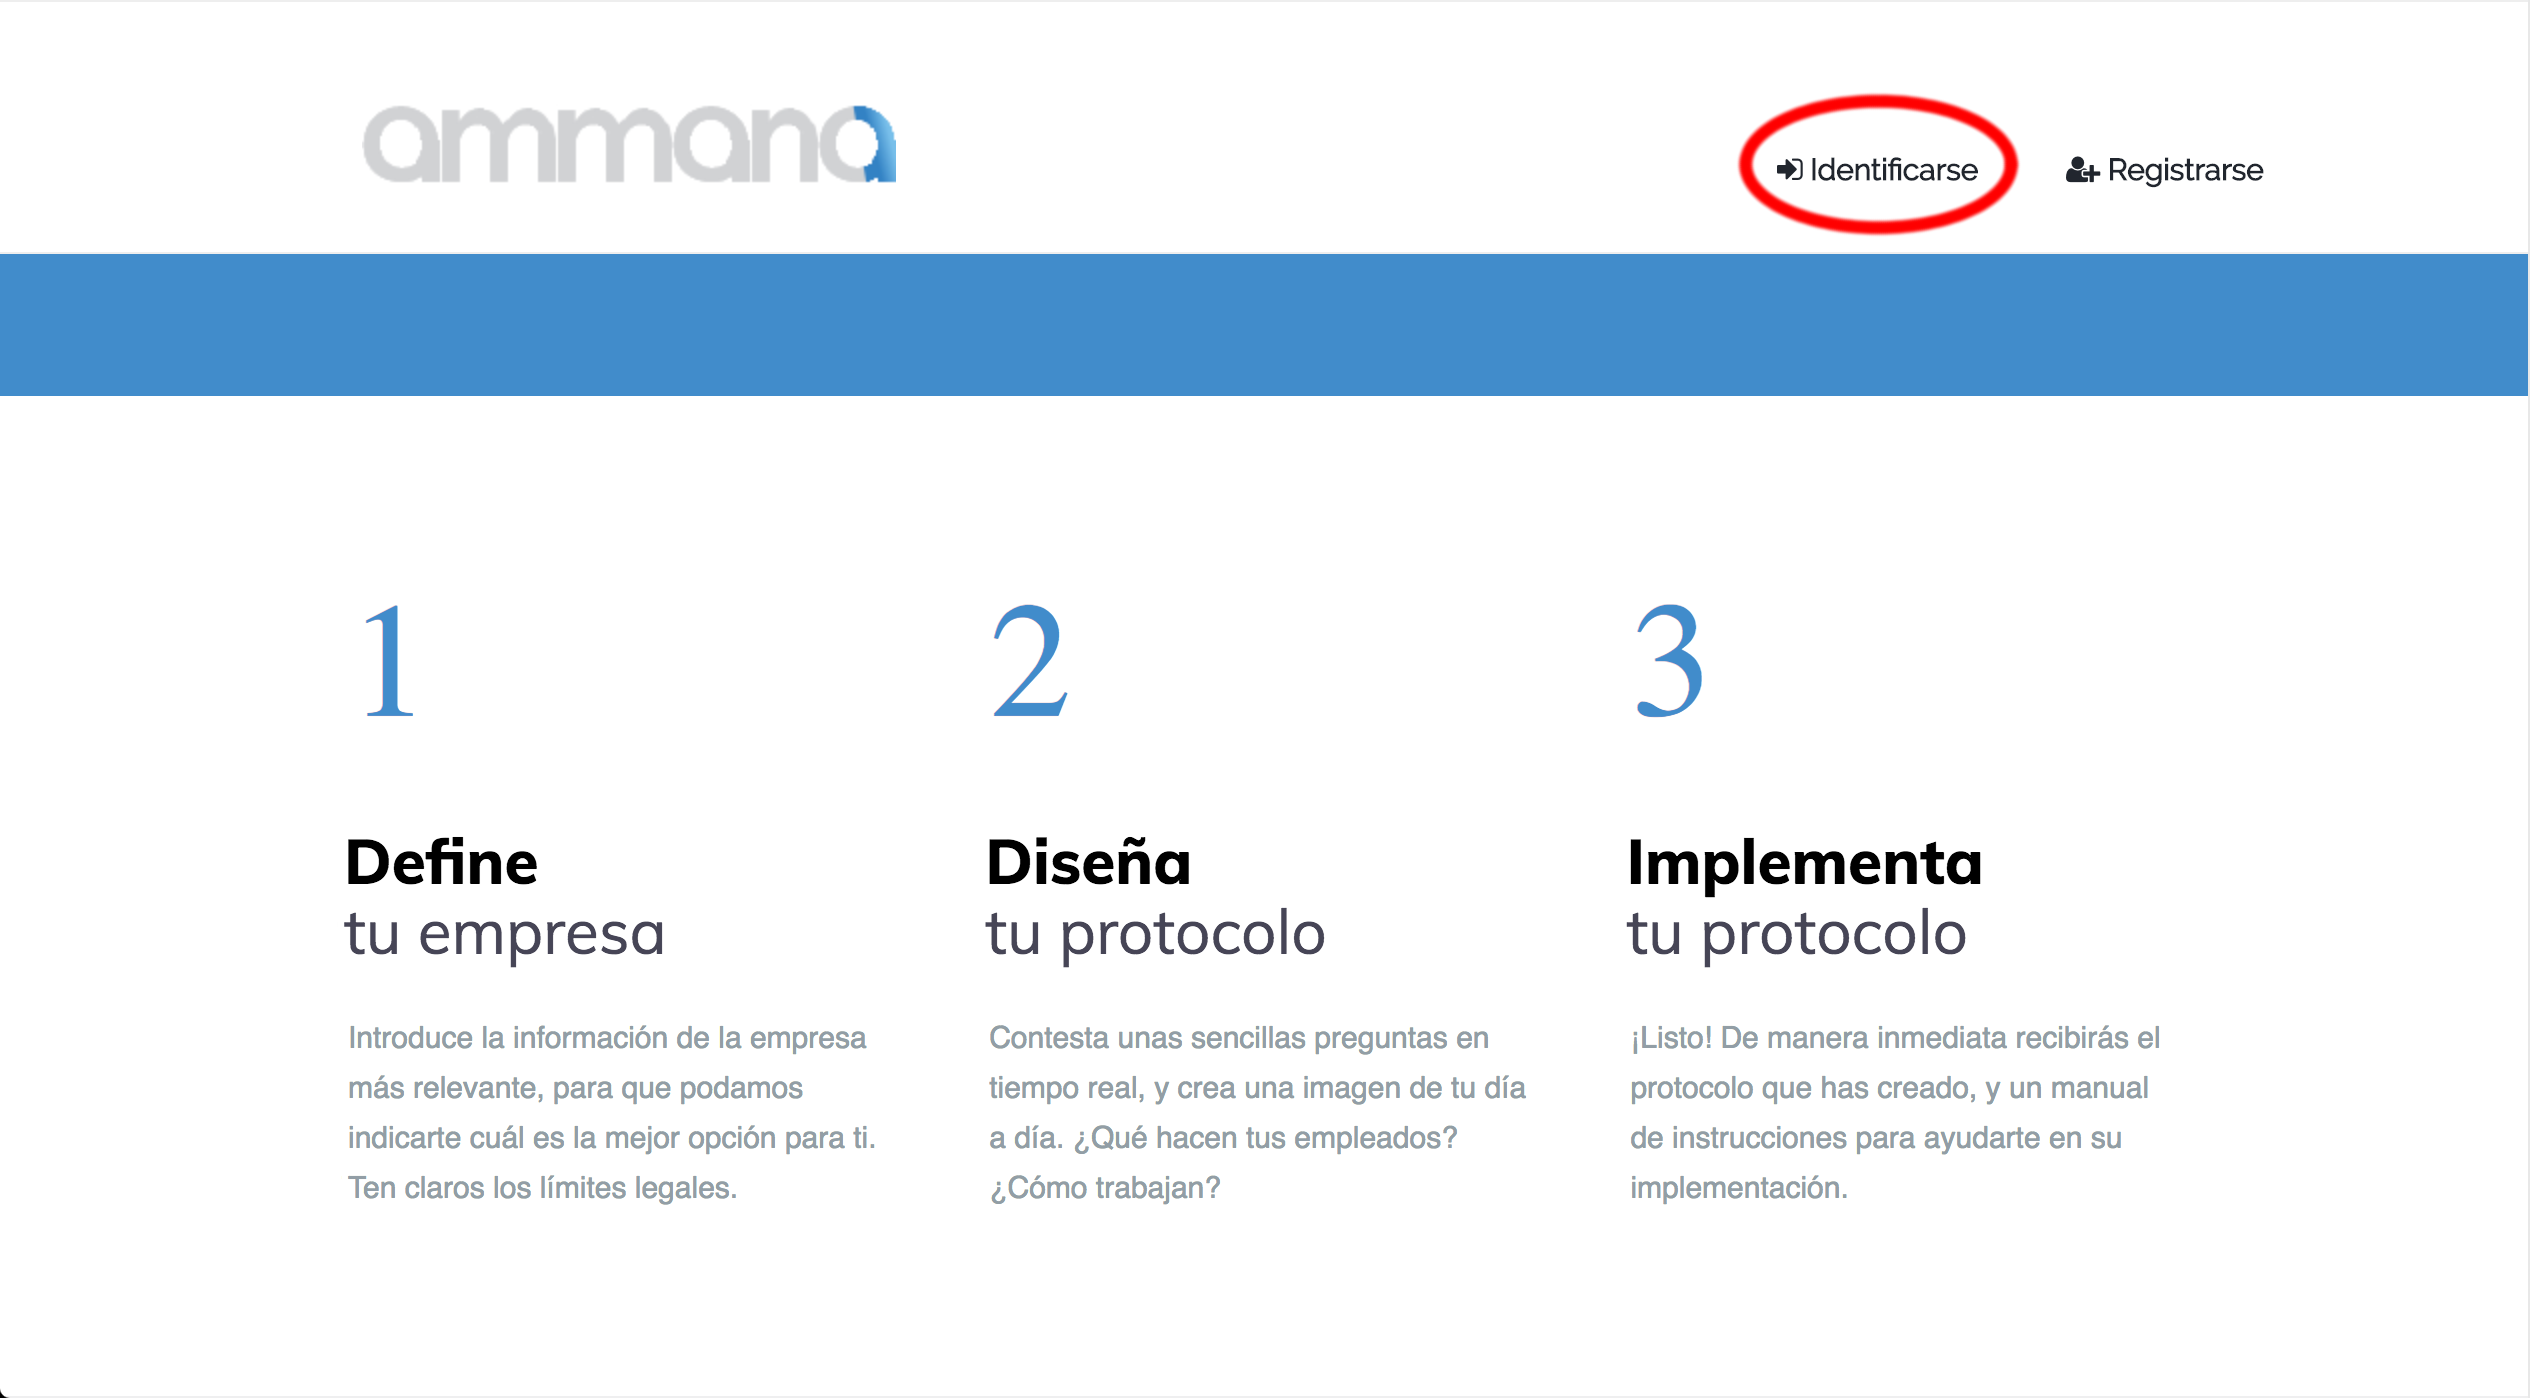
\includegraphics[width=1\linewidth]{login_button.png}%
            }
        \end{minipage}
        \item Introducir email y contraseña en el formulario de login:

            \medskip
            \begin{minipage}[t]{\linewidth}
            \raggedright
            \adjustbox{valign=t}{%
                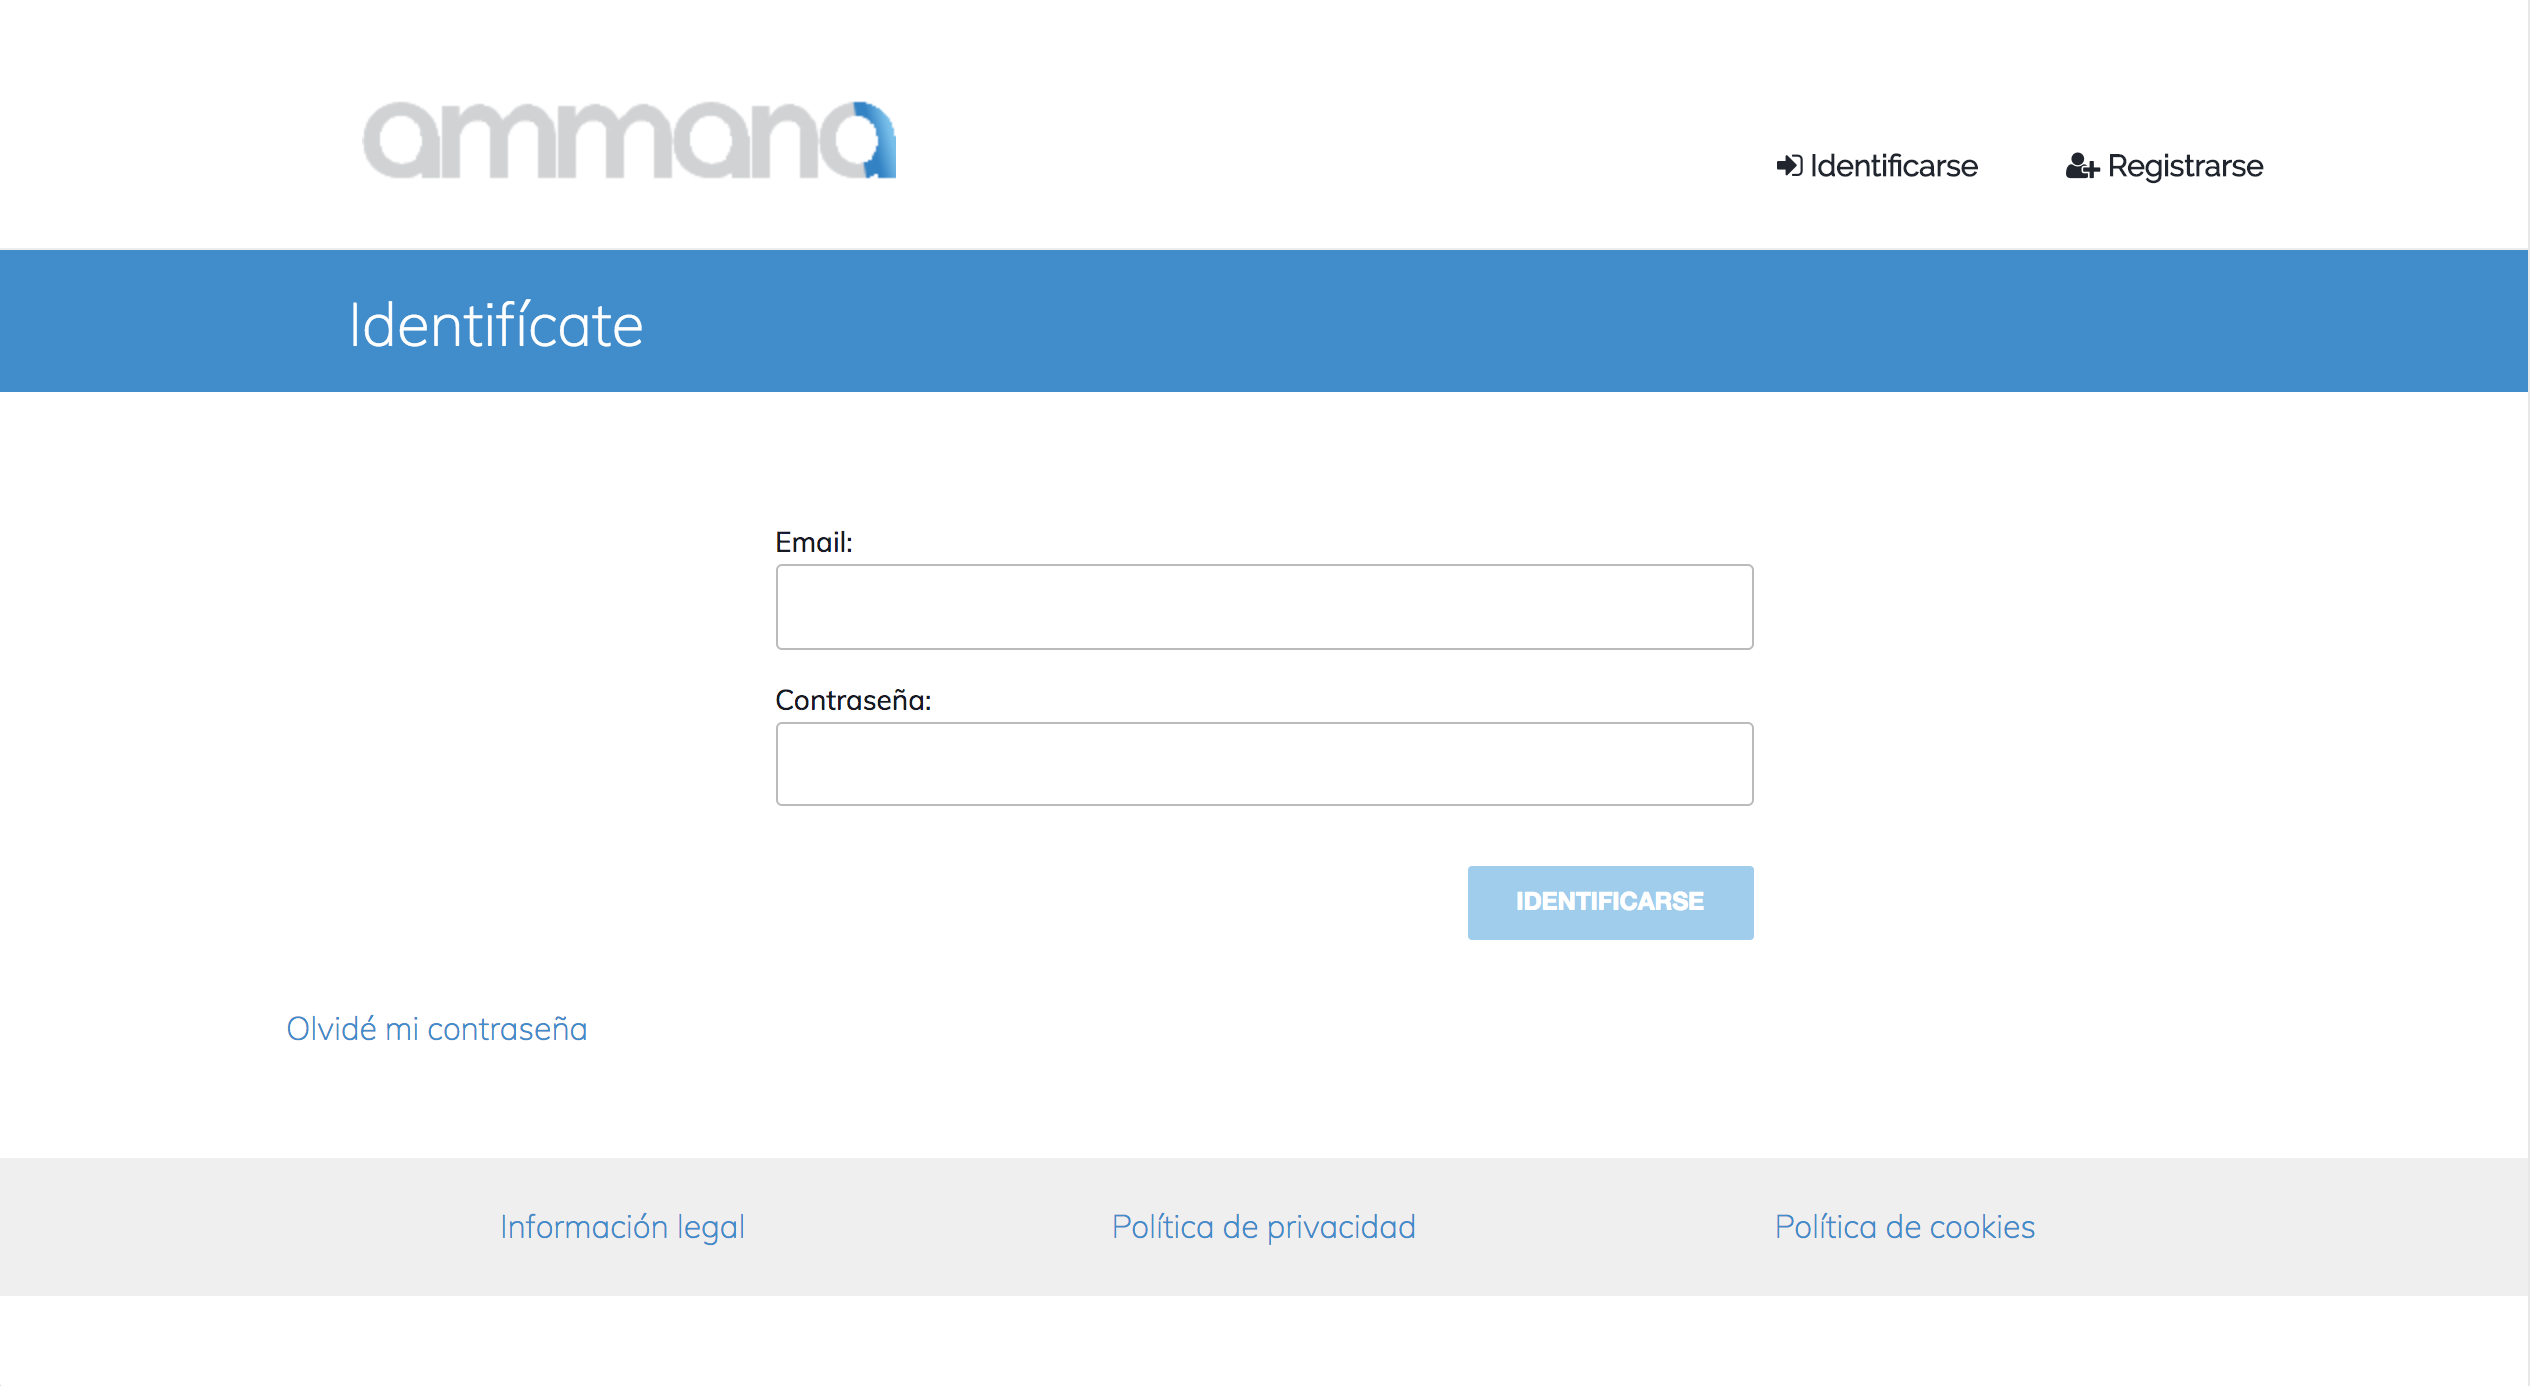
\includegraphics[width=1\linewidth]{login_form.png}%
            }
        \end{minipage}
    \end{steps}

%------------------------------------------------

    \subsection{URLs}

    ammana está publicado en ammana.es y protocololaboral.es

%------------------------------------------------

    \subsubsection{Cuentas de usuario}

    Cada usuario tiene una cuenta.
    Los usuarios se registran ellos solos.
    Existe la cuenta de administrador, que es especial. No se pueden registrar más cuentas de administración.

    \begin{figure}[H] % Example image
    \center{
\includegraphics[width=0.5\linewidth]{placeholder}}
    \caption{Example image.}
    \label{fig:speciation}
    \end{figure}

%------------------------------------------------

    \subsubsection{Registrar usuario}

    1) Ir a ammana.es
    2) Click en registrarse
    3) Introducir email y contraseña
    4) En dicho email se recibe correo de bienvenida
    5) Click en link de activación

%------------------------------------------------

    \section{Login}

    1) Ir a ammana.es
    2) Click en identificarse
    3) Introducir email y contraseña

%------------------------------------------------

    \subsection{Recuperar contraseña}

    1) Ir a ammana.es
    2) Click en identificarse
    3) Click en "Olvidé mi contraseña"
    4) Introducir email y click en "Enviar"
    5) En dicho email se recibe correo de establecer nueva contraseña
    6) Click en link
    7) Introducir nueva contraseña y clic en establecer

%------------------------------------------------

    \subsection{Modificar datos de perfil de usuario}

    1) Hacer login
    2) Clic en "Mi perfil"
    3) Modificar datos y clic en "actualizar"
    \begin{wrapfigure}{l}{0.4\textwidth} % Inline image example
      \begin{center}
        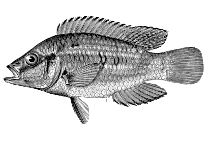
\includegraphics[width=0.38\textwidth]{fish}
      \end{center}
      \caption{Fish}
    \end{wrapfigure}
    Lorem ipsum...

%------------------------------------------------

    \subsubsection{Comprar protocolo}

    \begin{description}

        \item[First] \hfill \\
        Hacer login

        \item[Second] \hfill \\
        Clic en "Mis protocolos"

        \item[Third] \hfill \\
        Escoger protocolo en la lista bajo el epígrafe "Comprar protocolos"

        \item[Fourth] \hfill \\
        En el formulario, responder a todas las preguntas y clic en "Generar protocolo"

        \item[Fifth] \hfill \\
            Revisar las respuestas (modificarlas en su caso) y clic en "Confirmar"

        \item[Sixth] \hfill \\
        Clic en botón de Paypal y pagar.  Alternativamente pagar por transferencia bancaria.

    \end{description} 

%------------------------------------------------

    \subsubsection{Marcar protocolo como pagado}

    \begin{description}

        \item[First] \hfill \\
        Hacer login como administrador

        \item[Second] \hfill \\
        Clic en "Pedidos". Se muestran los pedidos que están sin cobrar.

        \item[Third] \hfill \\
        En el pedido correspondiente, clic en "Marcar como cobrado".

    \end{description} 

%------------------------------------------------

    \section{Conclusion}

    Esta es la conclusión

%------------------------------------------------

    \begin{thebibliography}{99}

        \bibitem[Figueredo and Wolf, 2009]{Figueredo:2009dg}
        Figueredo, A.~J. and Wolf, P. S.~A. (2009).
        \newblock Assortative pairing and life history strategy - a cross-cultural
          study.
        \newblock {\em Human Nature}, 20:317--330.
         
    \end{thebibliography}

    %----------------------------------------------------------------------------------------

\end{document}
